\chapter{Implementation details}
\label{ch:implementation}

\section{Structure}
\label{sec:structure}

\begin{figure}
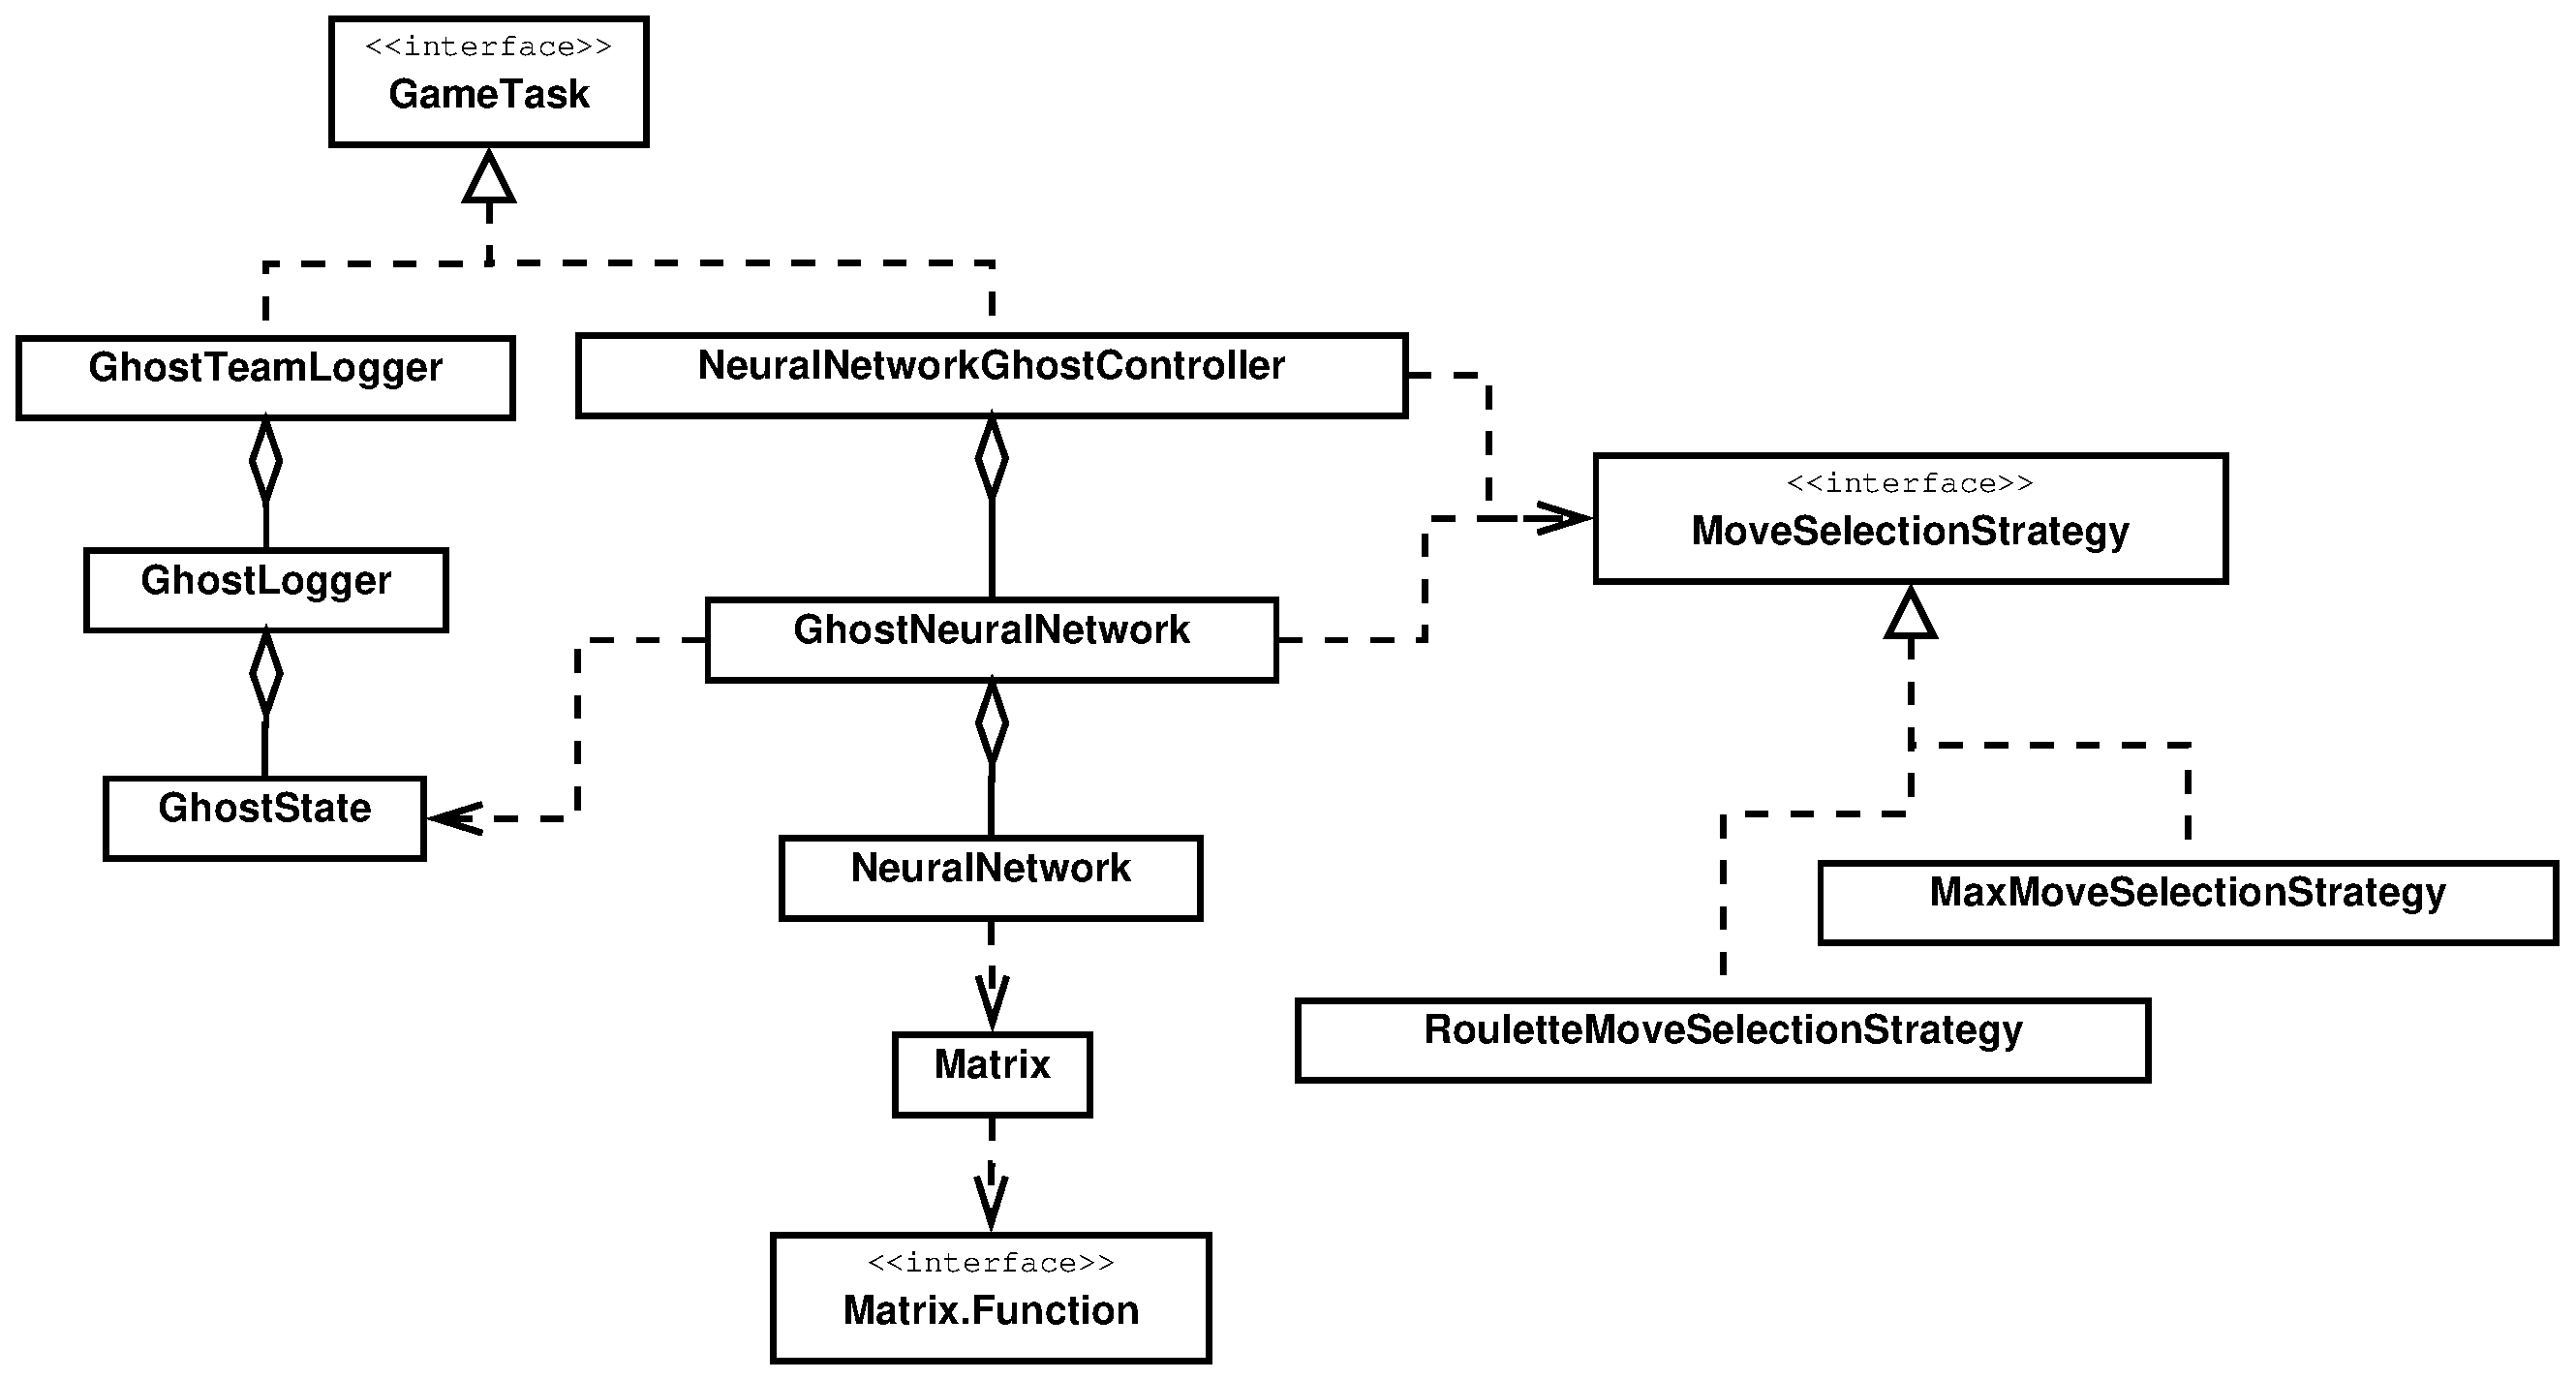
\includegraphics[width=\linewidth]{diagrams/project2}
\caption{Structure of the project}
\label{fig:project}
\end{figure}

Figure \ref{fig:project} shows the overall structure of the project.  The {\tt NeuralNetworkGhostController} class is the main part of the project: this implements the learning ghost controller, and the other classes and interfaces support it.  It uses four instances of the {\tt GhostNeuralNetwork} class, one for each of the ghosts; this class merely wraps the {\tt NeuralNetwork} class to give it ghost-specific functionality.  The implementation of the neural network algorithm is in the {\tt NeuralNetwork} class---the chosen method uses matrices (see Section \ref{sec:matlab} for more details) and therefore this class depends on the {\tt Matrix} class for matrix operations.  The {\tt Matrix} class is optimised for this specific neural network task, covered in section \ref{sec:efficiency}; this is the reason for not using an off-the-shelf matrix implementation.

As detailed at the end of section \ref{sec:nnalgorithm}, there is a choice involved in the move selection strategy: the \emph{Strategy} design pattern is employed so that different strategies---implementing the {\tt MoveSelectionStrategy} interface---can be chosen at run time.  The two methods of move selection mentioned in that section, picking the move with the maximum value versus picking a move with a probability proportional to its respective value, are implemented by the {\tt MaxMoveSelectionStrategy} and the {\tt RouletteMoveSelectionStrategy} classes respectively.

The input to the neural network is represented by the {\tt GhostState} class.  This class is also used by the {\tt GhostLogger} class to save ghost data to a file for evaluation purposes (see section \ref{sec:logging} for details).  The {\tt GhostTeamLogger} class holds a reference to four instances of this class, one for each ghost, to encapsulate the logging into one class.  It implements the {\tt GameTask} interface which was added to allow classes to be registered to get called every game tick.  The {\tt NeuralNetworkGhostController} class also implements this interface so that it can train each tick.

\section{Matrix efficiency improvements}
\label{sec:efficiency}

Much difficulty was encountered in implementing the neural network in Java.  It was realised that the implementation would have to be efficient, and so it was attempted to write it as such from the start.  However this proved rather difficult as there is much that can go wrong with such a complex programming task, and it is difficult to spot the location of errors: the neural network simply fails to converge and the reason for this is usually not apparent at all.

The implementation was therefore reattempted with the goal of matching the MATLAB code as closely as possible, with the simplest possible code.  This network was trained using data recorded for Blinky from a game against the {\tt Legacy} controller (containing 1169 data points) in order to demonstrate that it worked.  Then a series of optimisations were made one at a time, each time re-running the test on the same data so that any bugs could be picked up.  This helped localise the source of problems.  There follows a discussion of the optimisations made with Table \ref{tab:optimisations} showing the time saved by each optimisation.  This time was determined by training the network 10 times with the aforementioned data for each optimisation, running for 1000 iterations each time with 10 hidden nodes.  An average was then obtained for each, in order to discount effects such as JVM overhead and temporary demands on the processor by other processes.

\subsection{Na\"{i}ve implementation}

The matrix implementation used by the original code used a 2D ``jagged'' array to store the matrix data.  Internally, such an array consists of an array of pointers to a separate array for each row.  Thus to access an element in row 2, column 3 for example (with the code {\tt data[2][3]}) the JVM must find the second element in the main array, dereference the pointer it finds there to get the row array, and then find the third element in that array.

If iterating through the data in a row-major fashion, the Java compiler is not smart enough to store the row array in a temporary variable: doing this manually gives a speed increase.  Iterating in a column-major fashion can actually usurp the efforts of the processor cache if the data is large enough, which greatly hampers the performance.

\begin{lstlisting}[language=java,caption={Multiply code},captionpos=b,label=lst:naive,float]
for (int i = 0; i < op1.rows; i++)
{
    for (int j = 0; j < op2.columns; j++)
    {
        double sum = 0;

        for (int k = 0; k < op2.rows; k++)
        {
            sum += op1.data[i][k] * op2.data[k][j];
        }

        answer[i][j] = sum;
    }
}
\end{lstlisting}

As can be seen from listing \ref{lst:naive}, storing the matrix data like this is the easiest method to understand and therefore the easiest to program correctly; however there is obviously a need to improve the efficiency.

\subsection{An improved representation}

The first optimisation applied was to store the matrix data as a flat array, where each row is stored sequentially.  Thus, instead of accessing {\tt data[2][3]}, the programmer would access {\tt data[2 * numberOfColumns + 3]}.  Multiplication is much slower than repeated adding however, and an even greater saving can be made if adding is used when iterating over the data instead of multiplying.  Note in Listing \ref{lst:flatarray} how the indices to each part of the data are stored and multiplication is avoided.

\begin{lstlisting}[language=java,caption={Multiply code with flat arrays},captionpos=b,label=lst:flatarray,float]
int answerindex = 0, op1index = 0, op2index;

for (int i = 0; i < op1.rows; i++)
{
    for (int j = 0; j < op2.columns; j++)
    {
        double sum = 0;
        op2index = j;

        for (int k = 0; k < op2.rows; k++)
        {
            sum += op1.data[op1index + k] * op2.data[op2index];
            op2index += op2.columns;
        }

        answer[answerindex++] = sum;
    }

    op1index += op1.columns;
}
\end{lstlisting}

This is by far the biggest improvement in efficiency out of all the techniques applied, with the time taken to run 1000 iterations on the network dropping from 28.5 seconds to just 12.8---a saving of 15.7 seconds.

\subsection{Further enhancements}

The further enhancements optimise for specific patterns found in the neural network code that uses the matrix implementation (the neural network algorithm can be found in Appendix \ref{ap:matlab}).

Firstly, it was realised that many of the multiply operations were performed after first transposing one of the operands.  The transpose operation is quite slow as it involves iterating over the data and copying it to a new location, but it is really only rearranging the data---if instead the multiply function was to iterate over the operand data in such a way that mimicked one of the operands having been transposed, the transpose operation could be skipped entirely.  Therefore, two extra multiply functions were written: one which simulated transposing the first operand, and another which simulated transposing the second operand.  This improvement reduced the time taken by a further 2.7 seconds.

It was also noticed that often in the neural network algorithm, some matrix operation is performed such as multiplication or addition, then some function is applied to all of the elements of the resulting matrix.  The na\"{i}ve implementation has to iterate over all the data twice in this scenario, but a better approach would be to give the ability to apply the function to each element at the same time as the first operation is happening.  An interface was made to represent an element-wise function, and an argument was added to each of the element operator functions to accept an instance of this interface.  This optimisation reduced the over all time by a fifth of a second.

Other modifications were then made in the same vein, designed to avoid iterating over the data more times than is necessary.  Each step in the algorithm dealing with forward propagation, backward propagation and finally updating of the neural network weights was implemented in a custom function, resulting in the overall running time on the test data being reduced to just under 5 seconds.  This is a significant saving from the original 28.5 seconds.  Listings \ref{lst:before} and \ref{lst:after} show the neural network algorithm before and after optimisations respectively.

\begin{table}[ht]
\centering
\begin{tabular}{lcc}
\toprule
Description & Running time (s) & Saving (s) \\
\midrule
Na\"{i}ve implementation & 28.535 & --- \\
Flat array storage & 12.767 & 15.768 \\
Transpose / multiply shortcut & 10.080 & 2.687 \\
Element-wise function shortcut & 9.875 & 0.205 \\
Custom weights updating & 7.264 & 2.611 \\
Custom forward propagation & 5.254 & 2.010 \\
Custom hidden layer error calculation & 4.966 & 0.288 \\
Custom output error calculation & 4.946 & 0.02 \\
\bottomrule
\end{tabular}
\caption[Algorithm running time after various optimisations]{Algorithm running time after various optimisations: each line follows on from the previous, thus the last line is the cumulative effect of all the previous optimisations.}
\label{tab:optimisations}
\end{table}

\begin{lstlisting}[language=Java,caption={Neural network algorithm before optimisation},label=lst:before,captionpos=b,float]
a1 = Utilities.appendVertical(1, x.part(j, j, 1, -1).transpose());
a2 = Utilities.appendVertical(1, theta1.multiply(a1).apply(sig));
a3 = theta2.multiply(a2).apply(sig);

t = y.part(j, j, 1, -1).transpose();
d3 = t.subtract(a3).elementMultiply(a3.apply(sigd));

d2 = theta2.part(1, -1, 2, -1).transpose().multiply(d3)
		.elementMultiply(a2.part(2, -1, 1, 1).apply(sigd));

theta1 = theta1.add(d2.multiply(a1.transpose()).scale(learningRate));
theta2 = theta2.add(d3.multiply(a2.transpose()).scale(learningRate));
\end{lstlisting}

\begin{lstlisting}[language=Java,caption={Neural network algorithm after optimisation},label=lst:after,captionpos=b,float]
a1 = x.getRowAsColumn(j);
a2 = calculateLayer(theta1, a1);
a3 = calculateLayer(theta2, a2);

t = y.getRowAsColumn(j);

d3 = calculateOutputError(t, a3);
d2 = calculateHiddenError(theta2, d3, a2);

updateWeights(theta1, d2, a1, learningRate);
updateWeights(theta2, d3, a2, learningRate);
\end{lstlisting}
